\documentclass[14pt,pdf,hyperref={unicode}]{beamer}

% \documentclass[aspectratio=43]{beamer}
% \documentclass[aspectratio=1610]{beamer}
% \documentclass[aspectratio=169]{beamer}

\usepackage{lmodern}

% подключаем кириллицу 
\usepackage[T2A]{fontenc}
\usepackage[utf8]{inputenc}
\usepackage{listings}
\usepackage{graphicx}
\usepackage{hyperref}

% отключить клавиши навигации
\setbeamertemplate{navigation symbols}{}

% тема оформления
\usetheme{CambridgeUS}

% цветовая схема
\usecolortheme{seahorse}

\definecolor{light-gray}{gray}{0.90}

\lstset{basicstyle=\ttfamily,breaklines=true}

\title{Семинар №12}   
\subtitle{ФАКИ 2015}
\author{Бирюков В. А.} 
\date{\today} 
% \logo{
\includegraphics[height=5mm]{images/logo.png}\vspace{-7pt}}

\begin{document}

\lstset{language=C}

% титульный слайд
\begin{frame}
\titlepage
\end{frame} 



\defverbatim[colored]\makeset{
\begin{lstlisting}[language=C++,basicstyle=\ttfamily,keywordstyle=\color{blue},
                stringstyle=\color{red}\ttfamily]
void make_set(int X) {
  parent[X] = X;
}
\end{lstlisting}
}

\lstset{
  language=C,                % choose the language of the code
  keywordstyle=\color{blue},
  numbers=none,                   % where to put the line-numbers
  stepnumber=1,                   % the step between two line-numbers.        
  numbersep=5pt,                  % how far the line-numbers are from the code
  backgroundcolor=\color{light-gray},  % choose the background color. You must add \usepackage{color}
  showspaces=false,               % show spaces adding particular underscores
  showstringspaces=false,         % underline spaces within strings
  showtabs=false,                 % show tabs within strings adding particular underscores
  tabsize=2,                      % sets default tabsize to 2 spaces
  captionpos=b,                   % sets the caption-position to bottom
  breaklines=true,                % sets automatic line breaking
  breakatwhitespace=true,         % sets if automatic breaks should only happen at whitespace
}



\section{Связный список}
\begin{frame}
\begin{center}
\begin{beamercolorbox}[sep=8pt,center]{part
title}
\usebeamerfont{part title}\insertsection
\end{beamercolorbox}
\end{center}
\end{frame}



\begin{frame}[fragile]
\frametitle{Связный список} 
\begin{center}
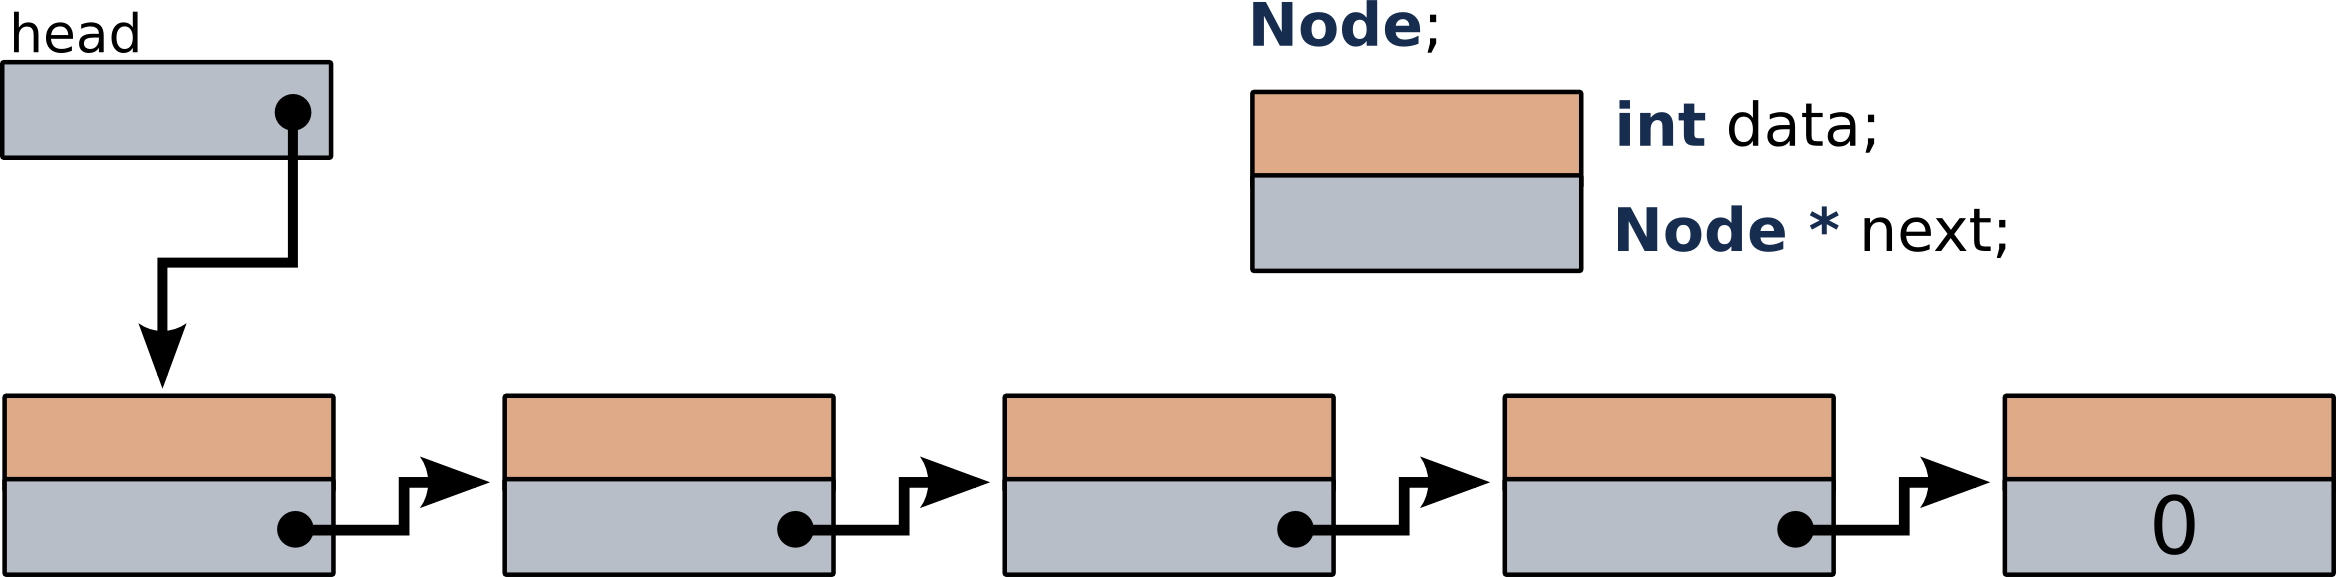
\includegraphics[width=0.99\linewidth]{images/list_initial.png}
\end{center}
\end{frame}


\begin{frame}[fragile]
\frametitle{Связный список} 
\framesubtitle{Обход связного списка - 1} 
\begin{center}
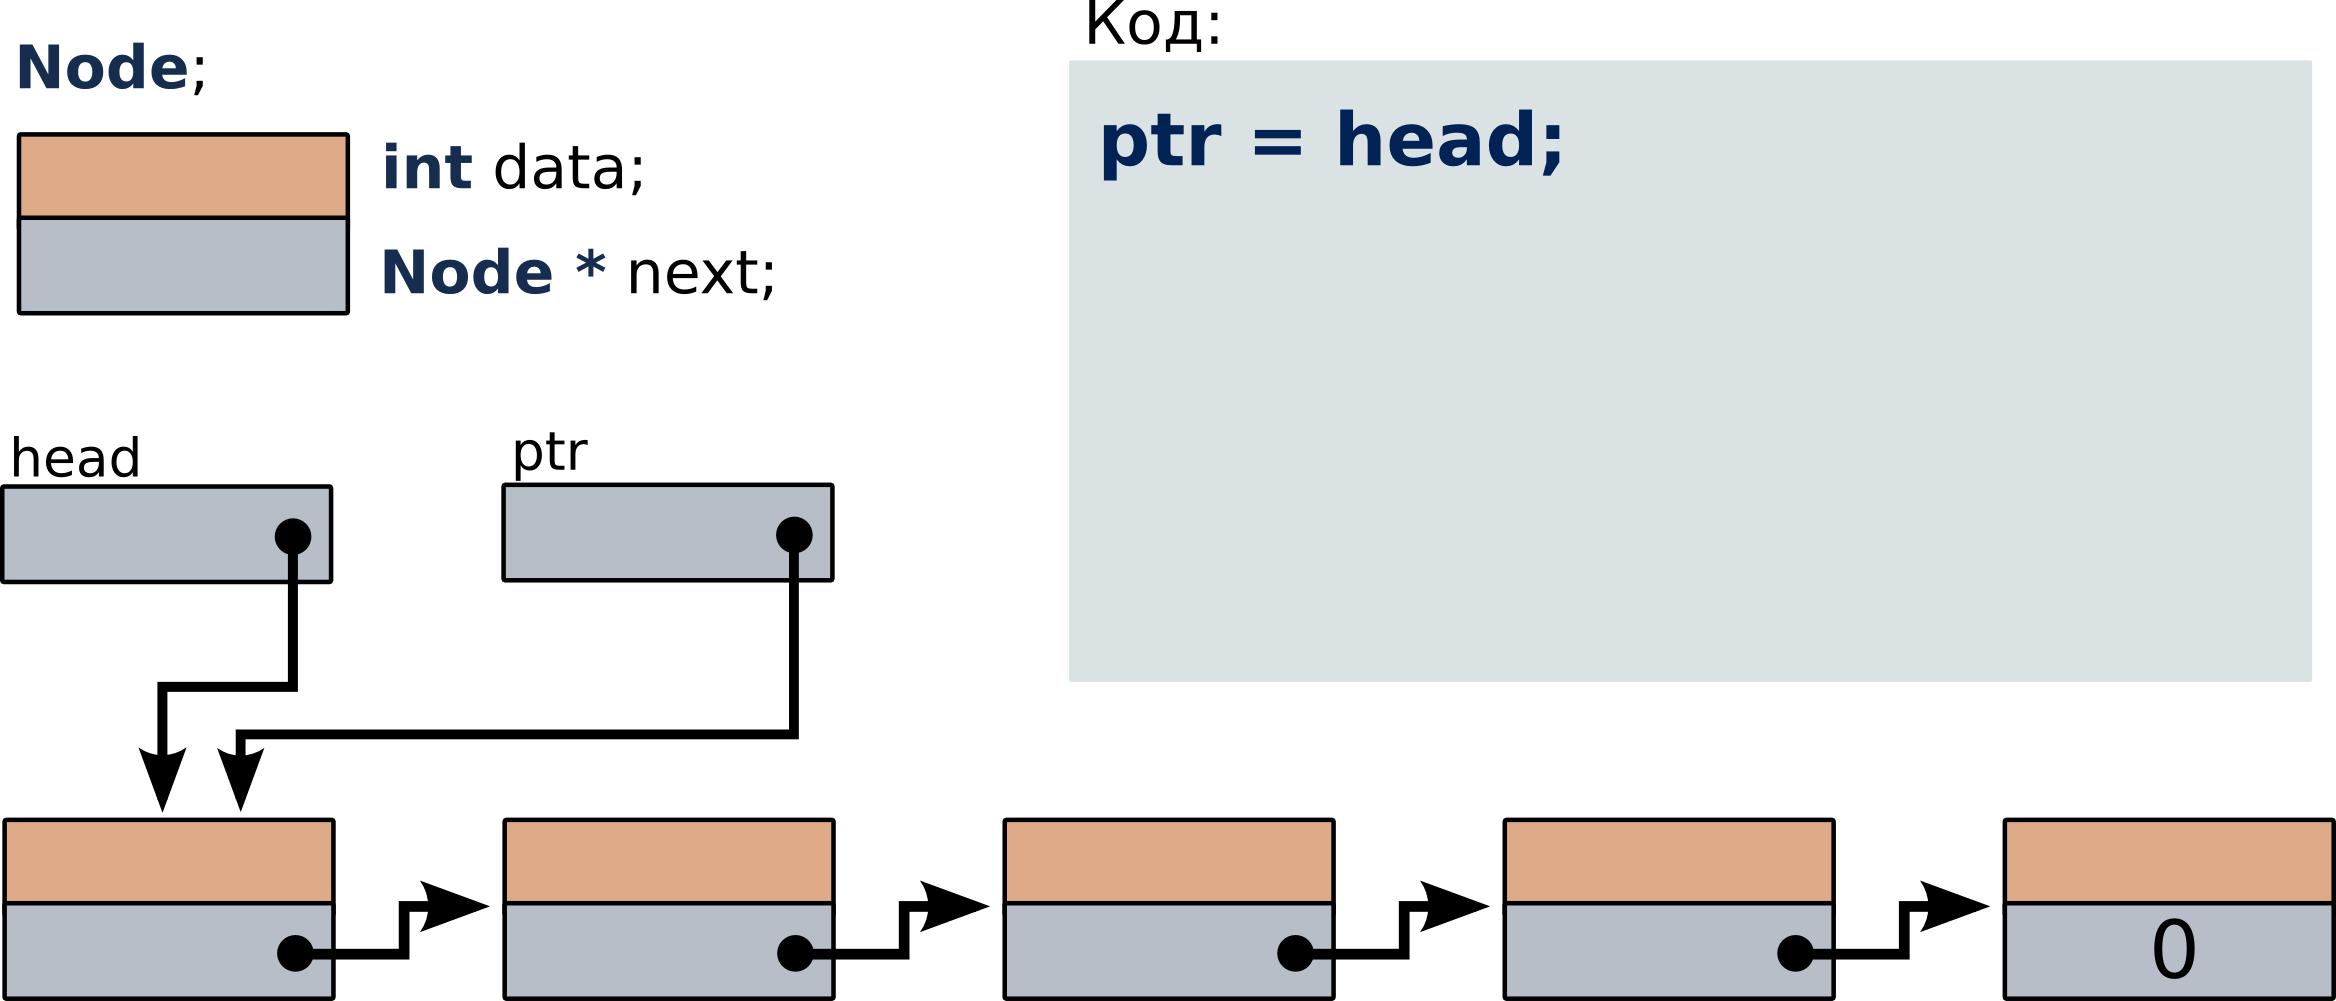
\includegraphics[width=0.99\linewidth]{images/list_traversal_1.png}
\end{center}
\end{frame}
\begin{frame}[fragile]
\frametitle{Связный список} 
\framesubtitle{Обход связного списка - 2} 
\begin{center}
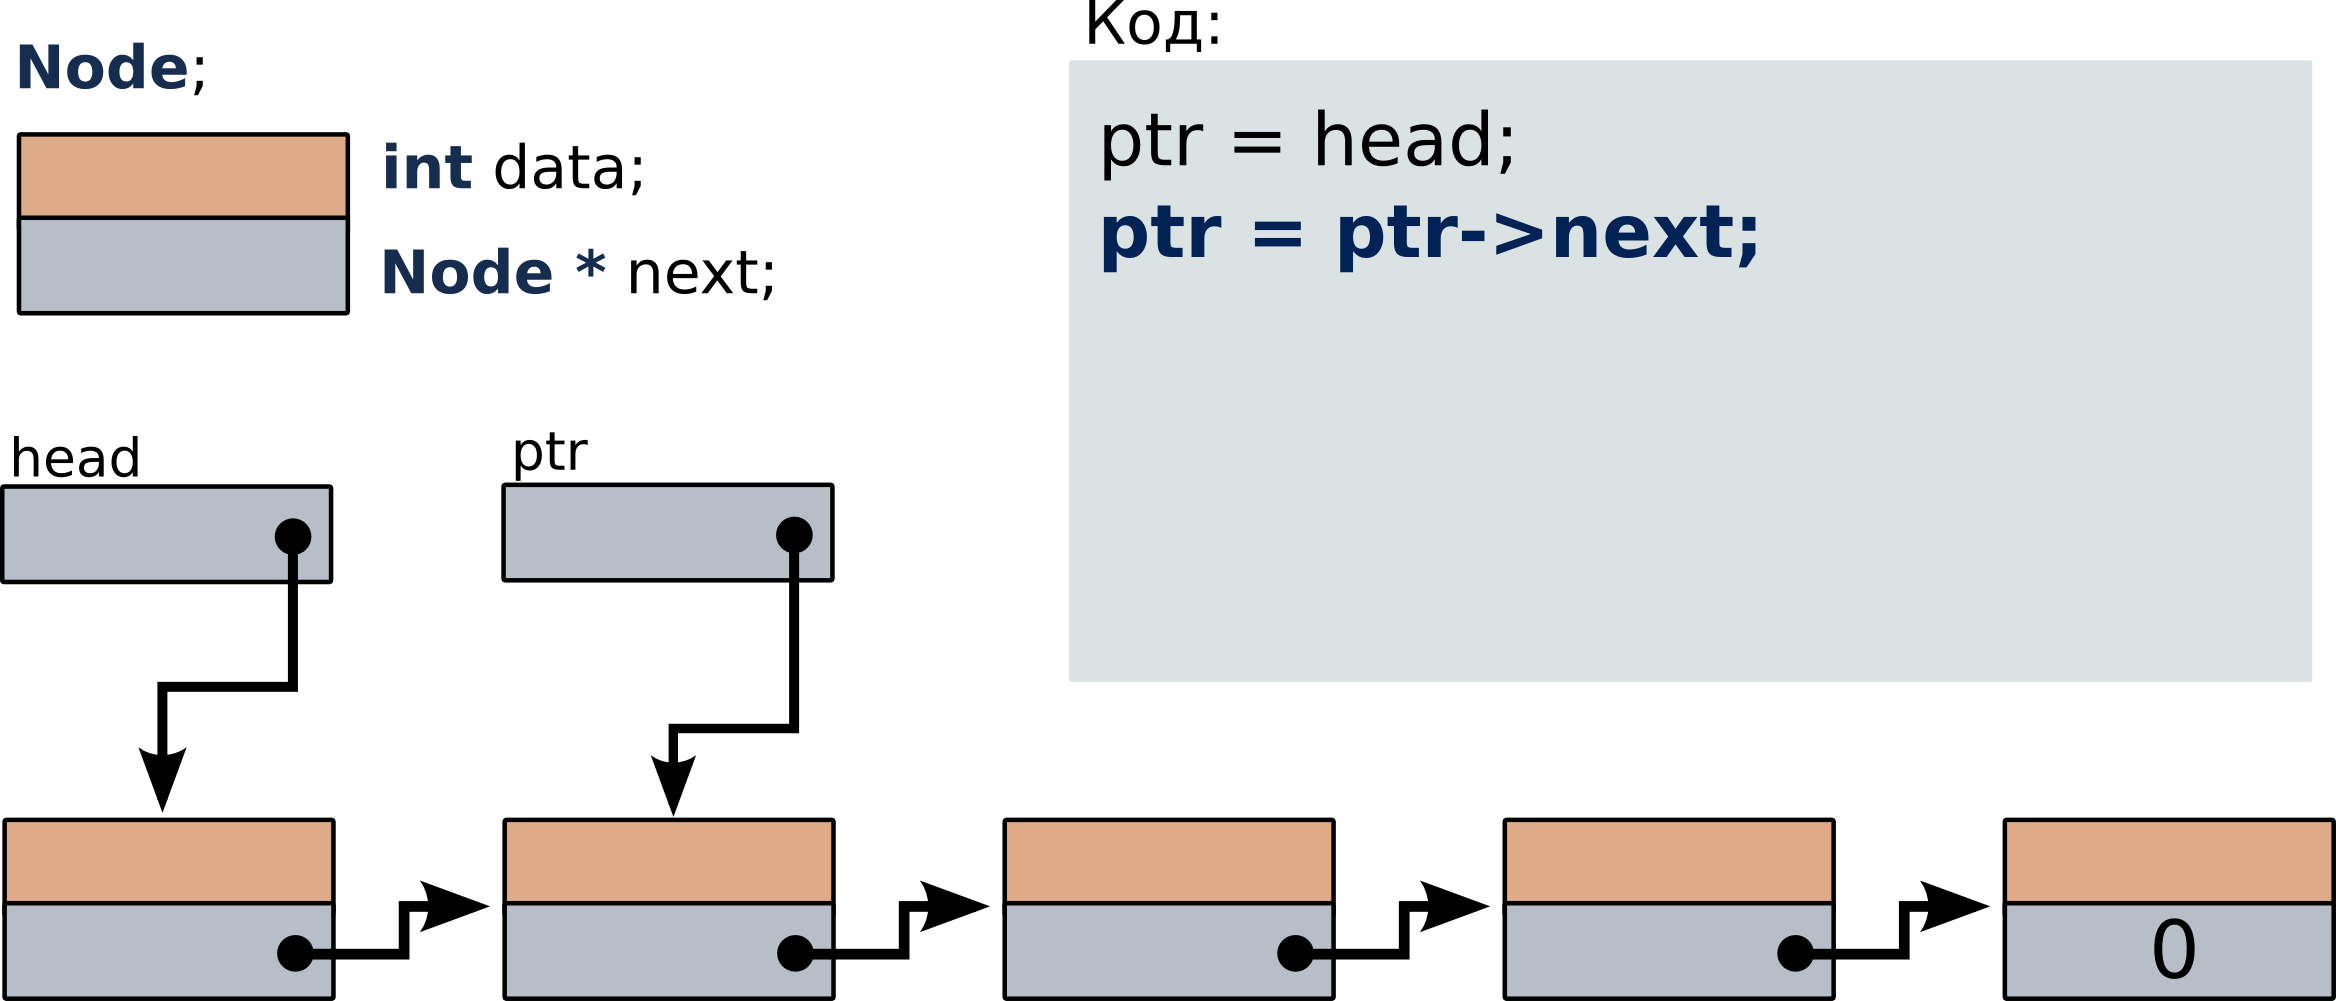
\includegraphics[width=0.99\linewidth]{images/list_traversal_2.png}
\end{center}
\end{frame}
\begin{frame}[fragile]
\frametitle{Связный список} 
\framesubtitle{Обход связного списка - 3} 
\begin{center}
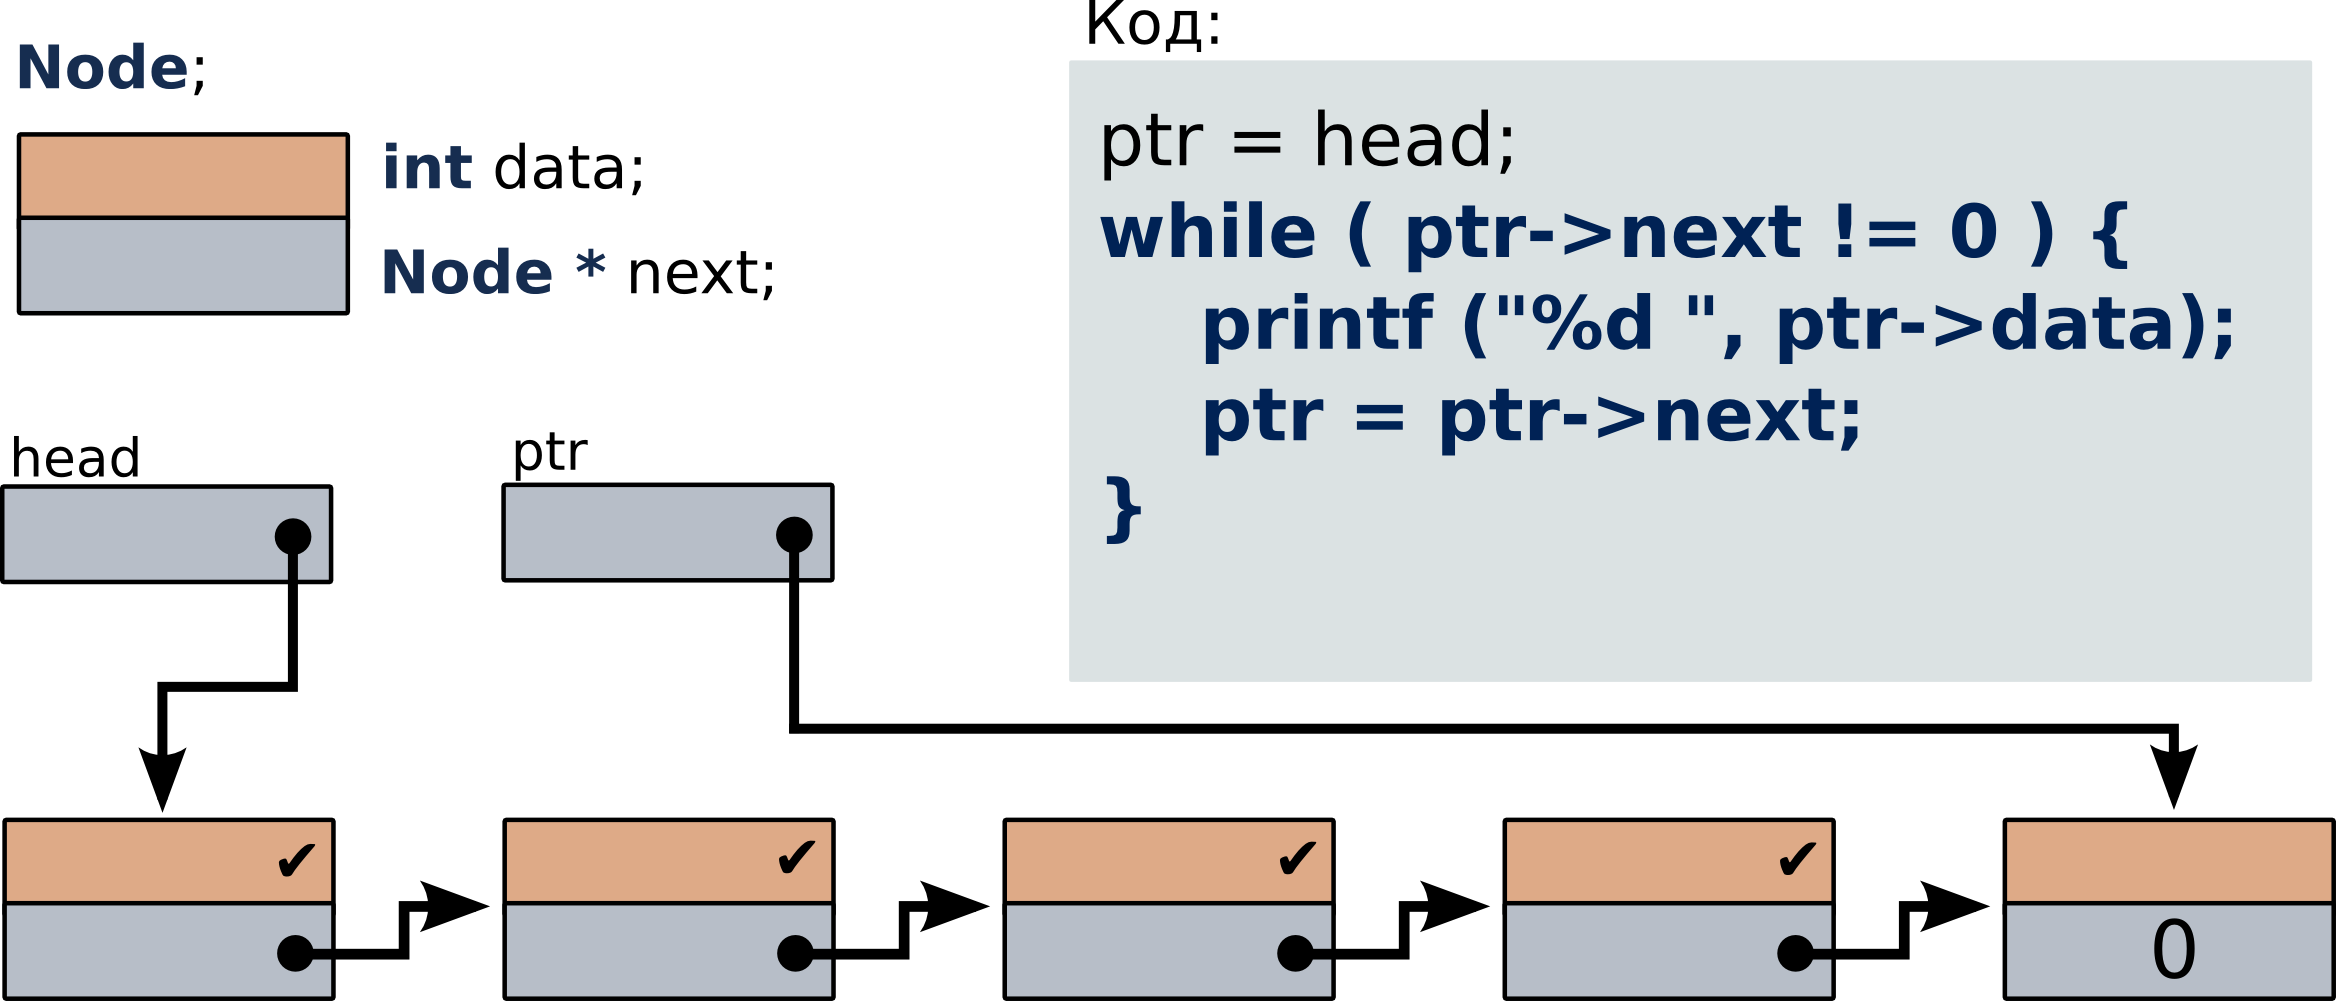
\includegraphics[width=0.99\linewidth]{images/list_traversal_3.png}
\end{center}
\end{frame}

\begin{frame}[fragile]
\frametitle{Связный список} 
\framesubtitle{Удаление элемента списка - 1} 
\begin{center}
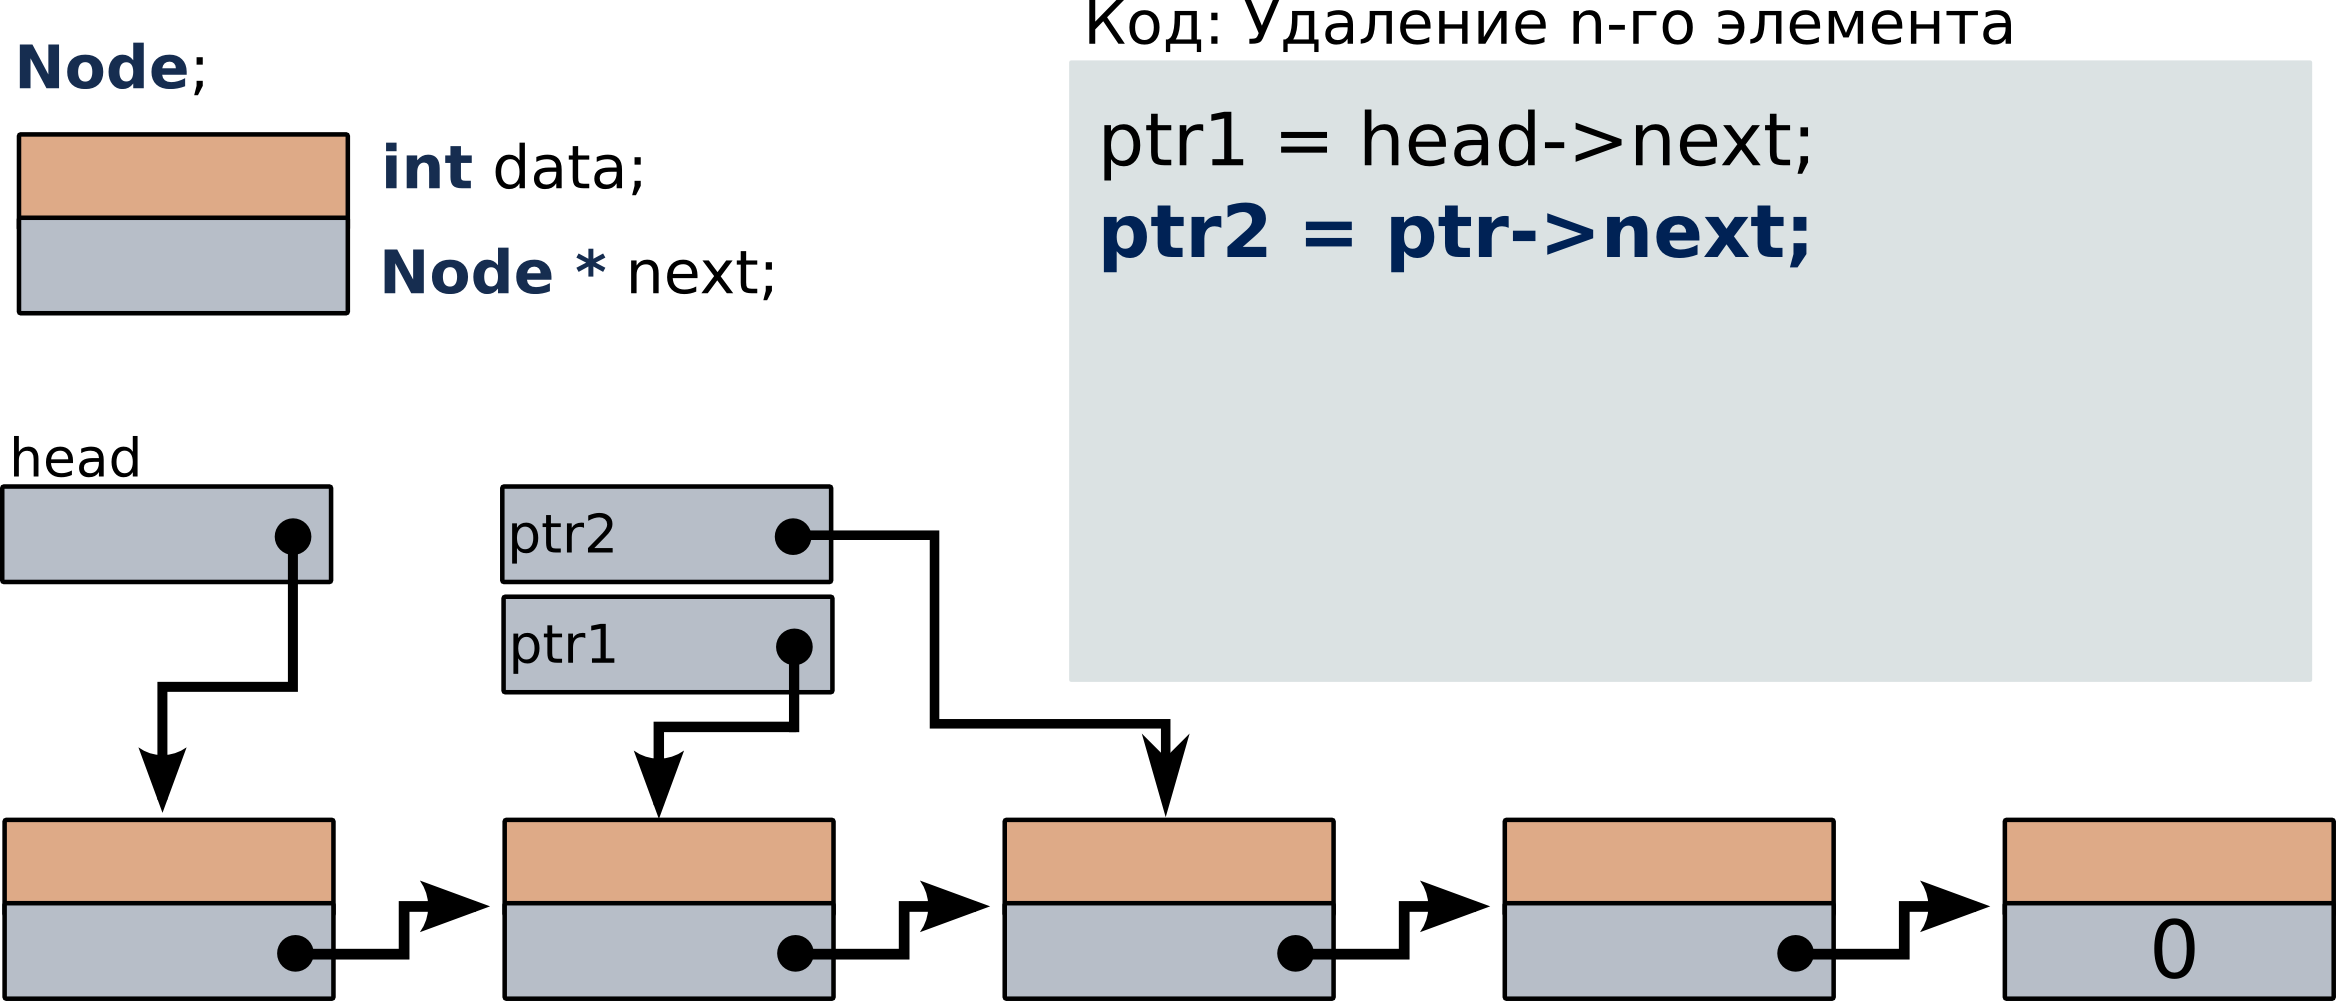
\includegraphics[width=0.99\linewidth]{images/list_delete_1.png}
\end{center}
\end{frame}
\begin{frame}[fragile]
\frametitle{Связный список} 
\framesubtitle{Удаление элемента списка - 2} 
\begin{center}
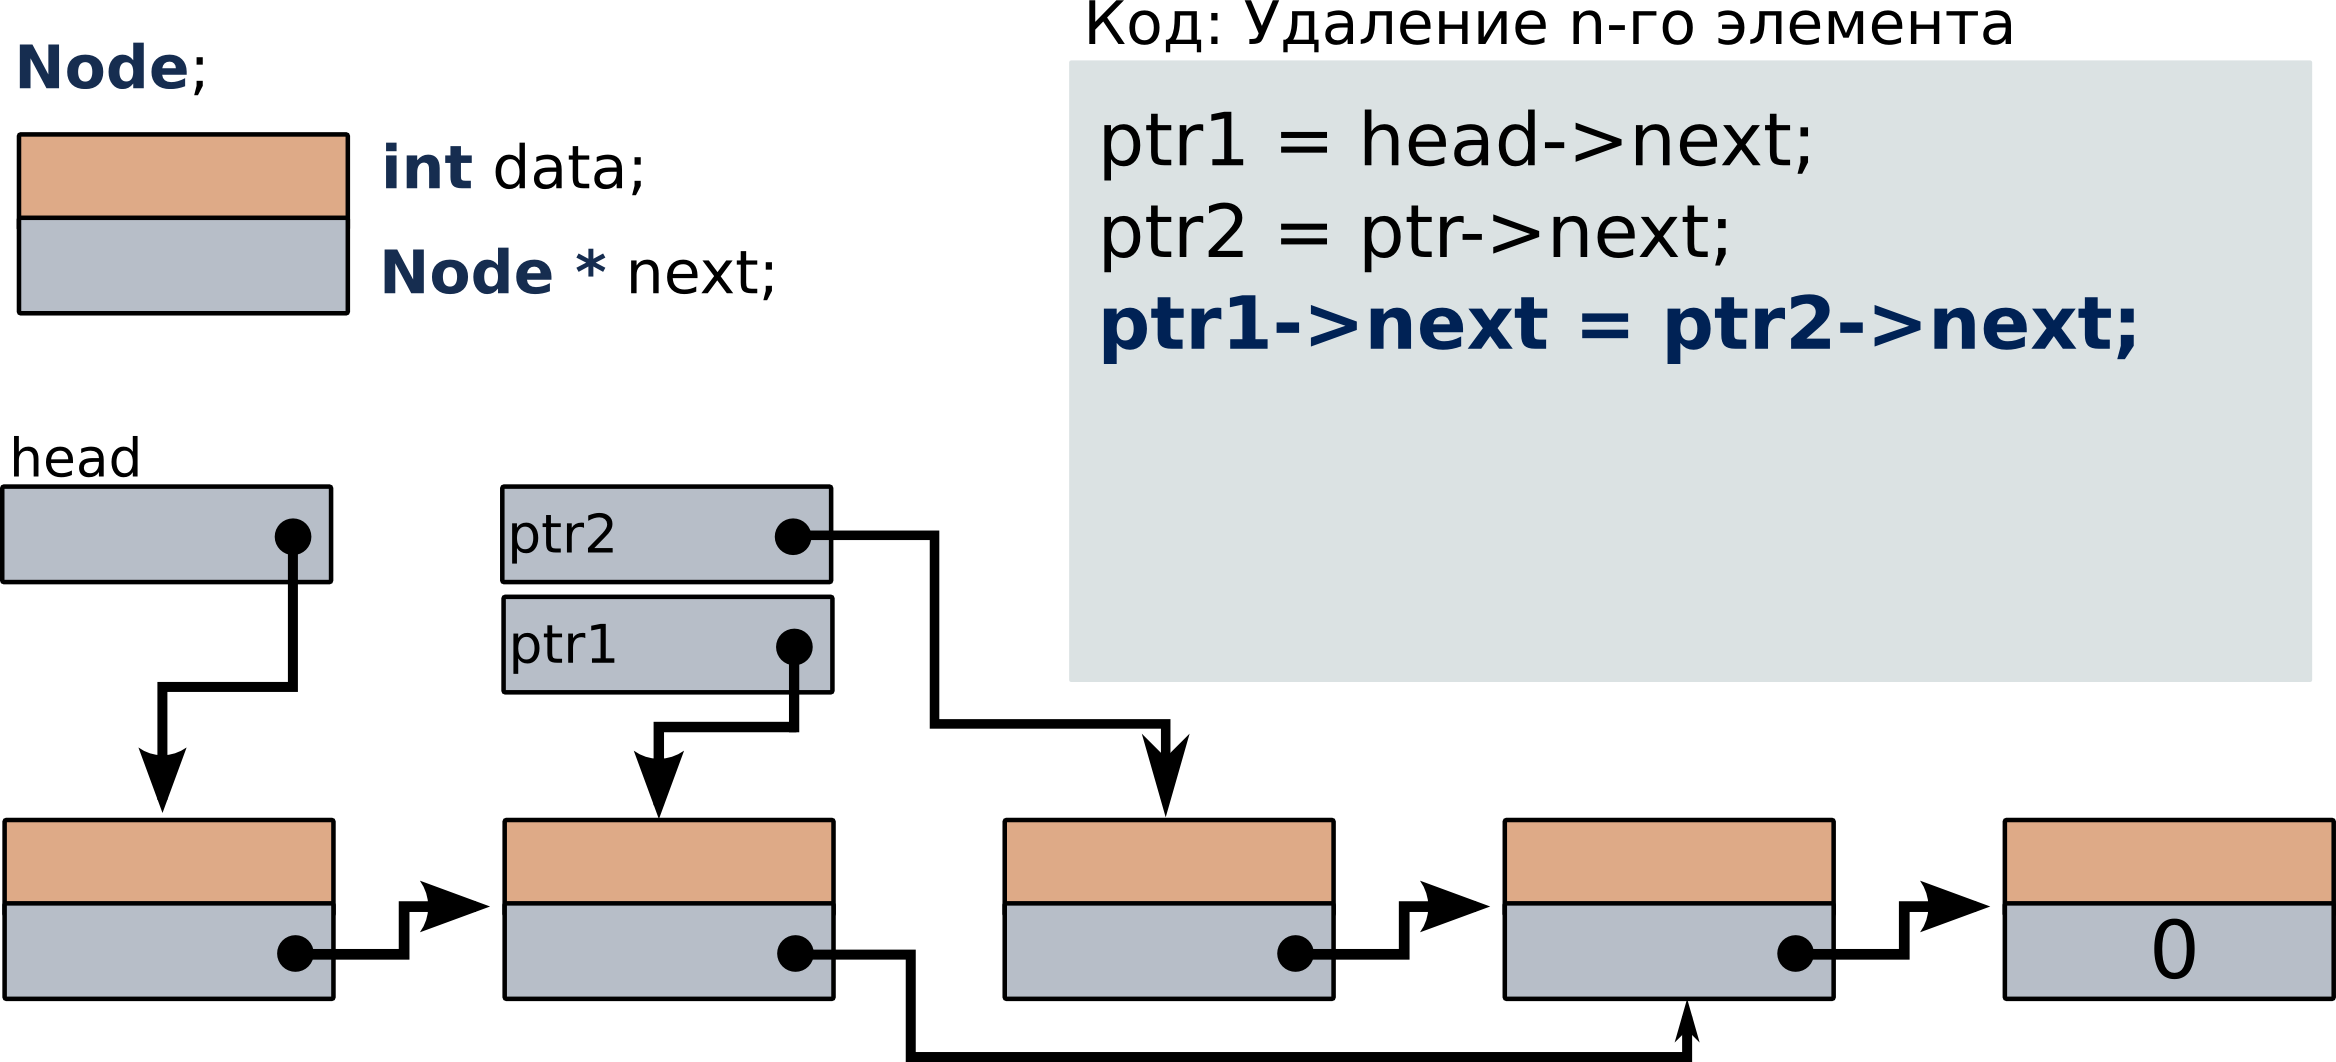
\includegraphics[width=0.99\linewidth]{images/list_delete_2.png}
\end{center}
\end{frame}
\begin{frame}[fragile]
\frametitle{Связный список} 
\framesubtitle{Удаление элемента списка - 3} 
\begin{center}
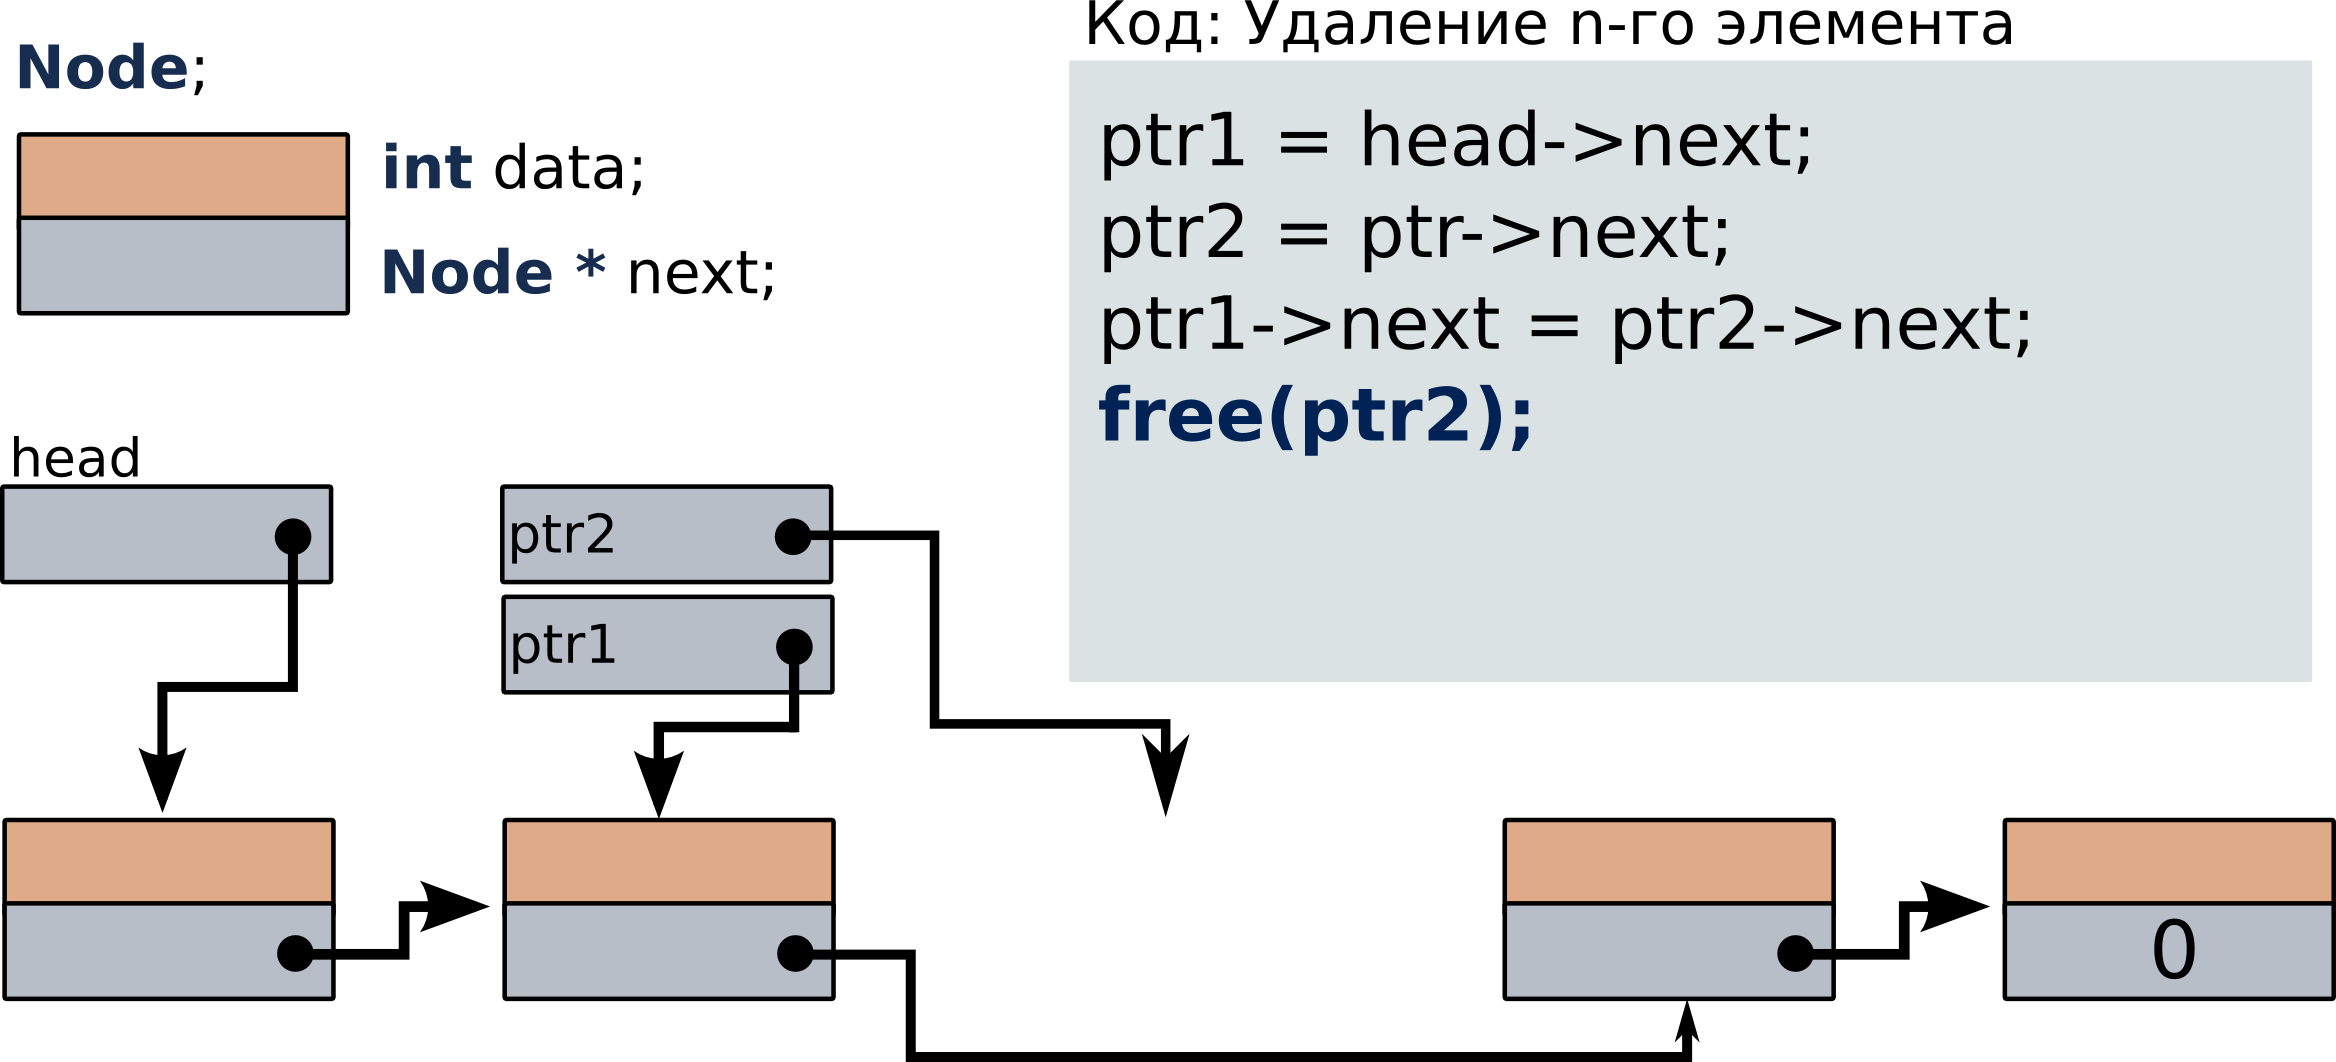
\includegraphics[width=0.99\linewidth]{images/list_delete_3.png}
\end{center}
\end{frame}




\section{Двоичные деревья поиска}
\begin{frame}
\begin{center}
\begin{beamercolorbox}[sep=8pt,center]{part
title}
\usebeamerfont{part title}\insertsection
\end{beamercolorbox}
\end{center}
\end{frame}

\begin{frame}[fragile]
\frametitle{Двоичные деревья} 
\begin{center}
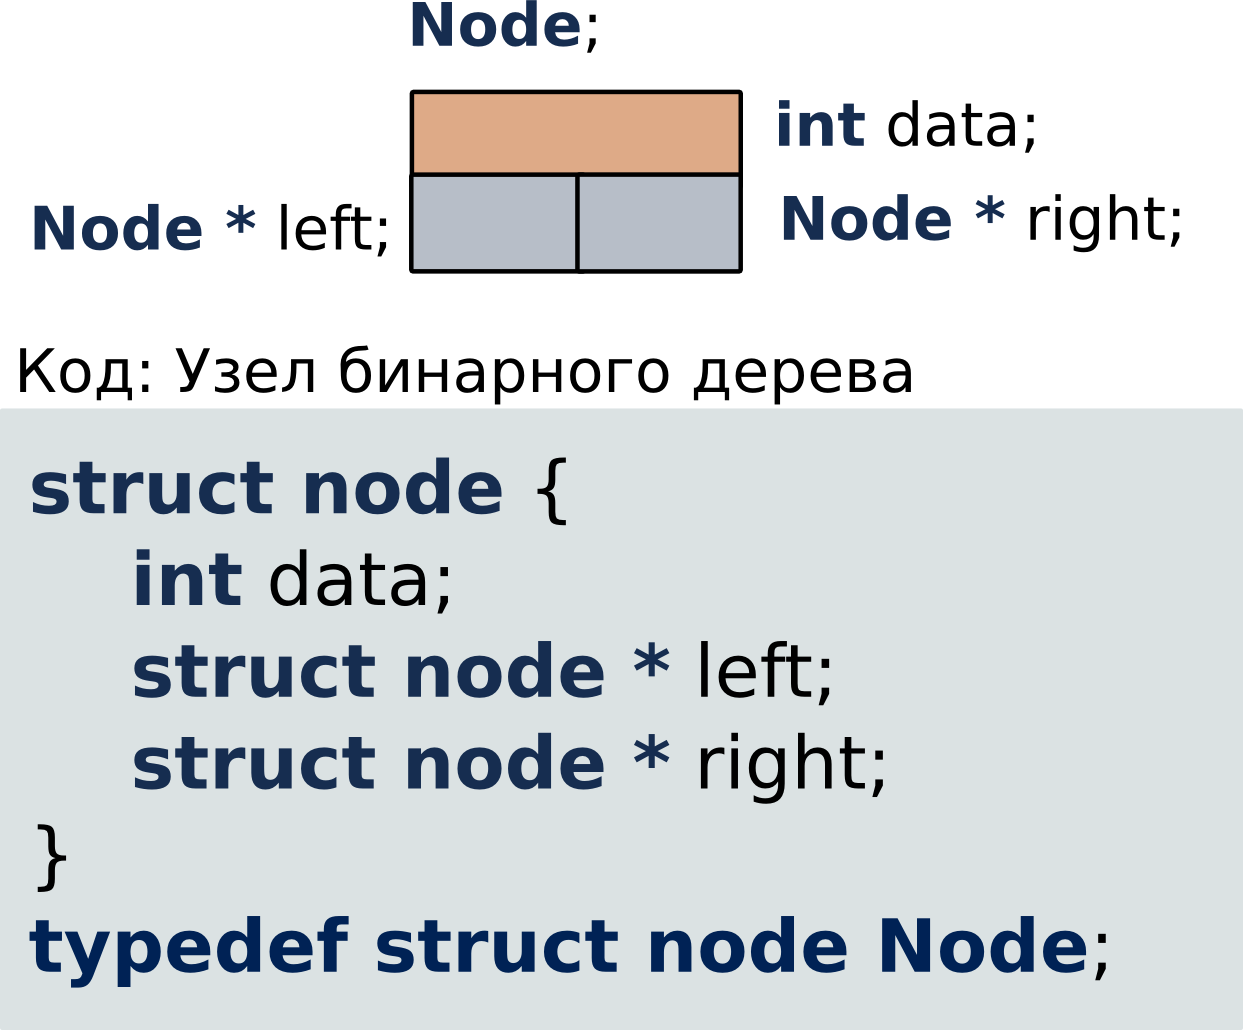
\includegraphics[width=0.6\linewidth]{images/bintree_initial.png}
\end{center}
\end{frame}
\begin{frame}[fragile]
\frametitle{Двоичные деревья}  
\begin{center}
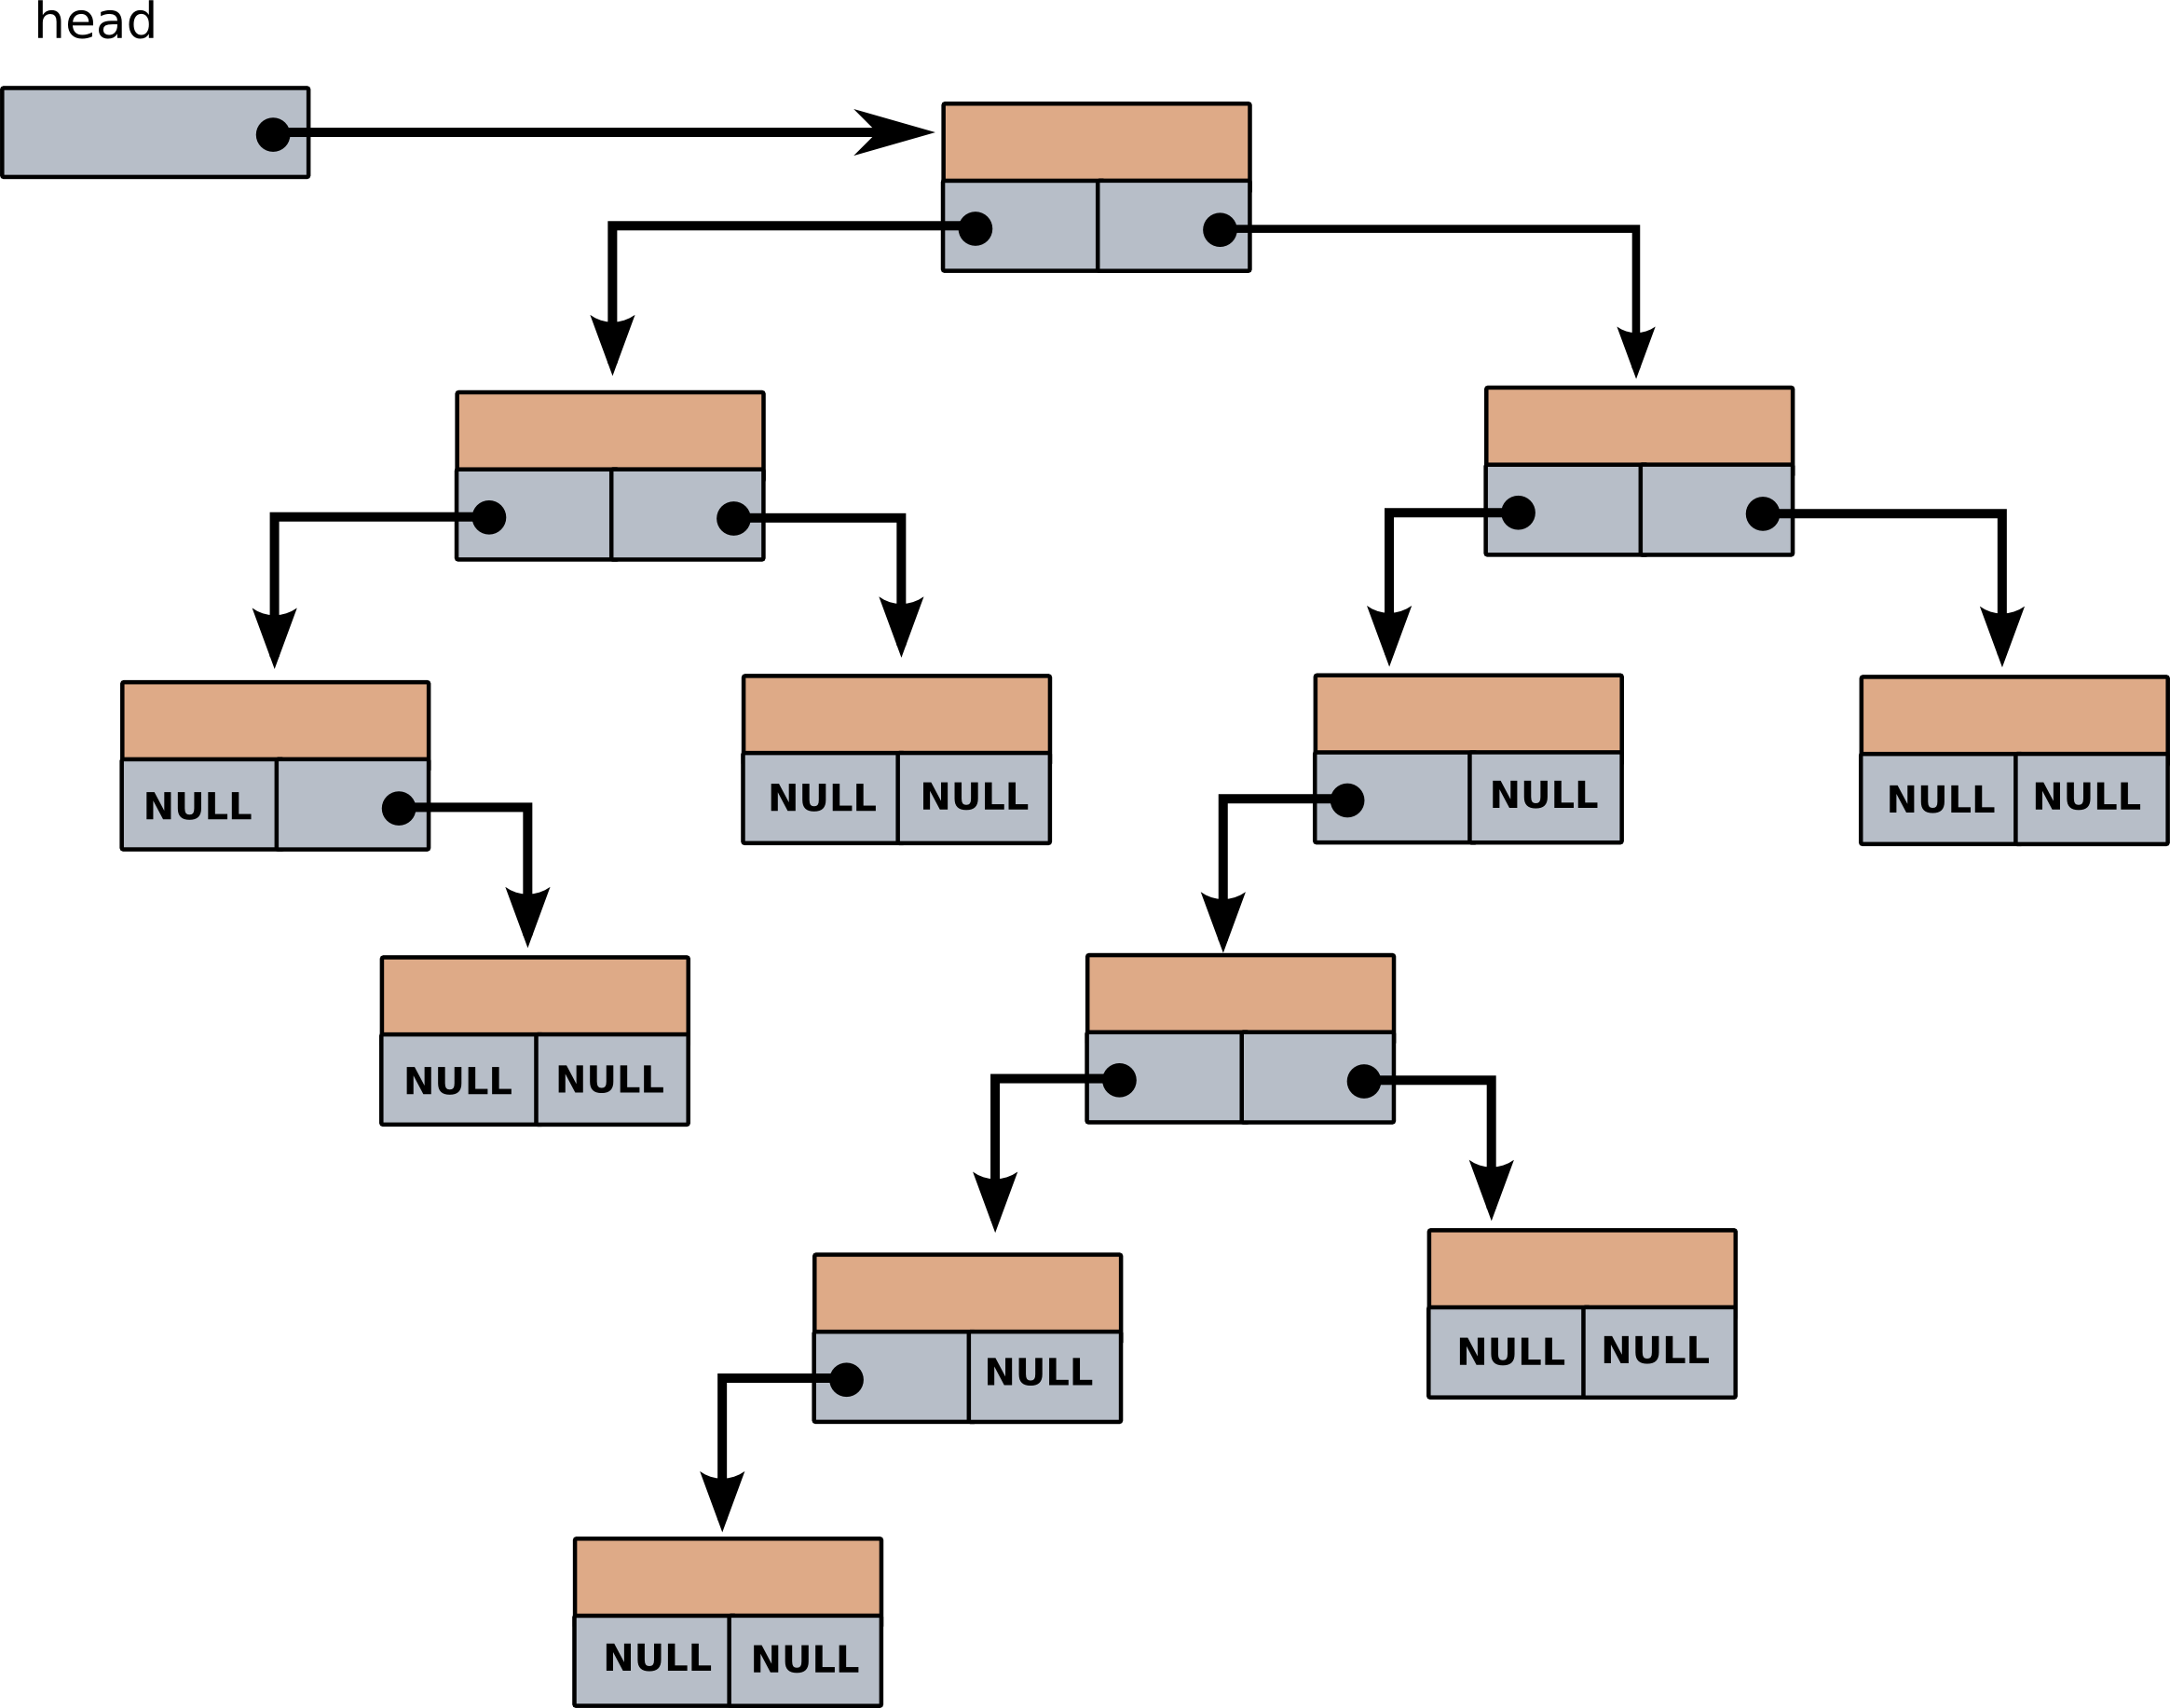
\includegraphics[width=0.75\linewidth]{images/bintree_initial_2.png}
\end{center}
\end{frame}

\begin{frame}[fragile]
\frametitle{Двоичные деревья (обход)}  
\begin{center}
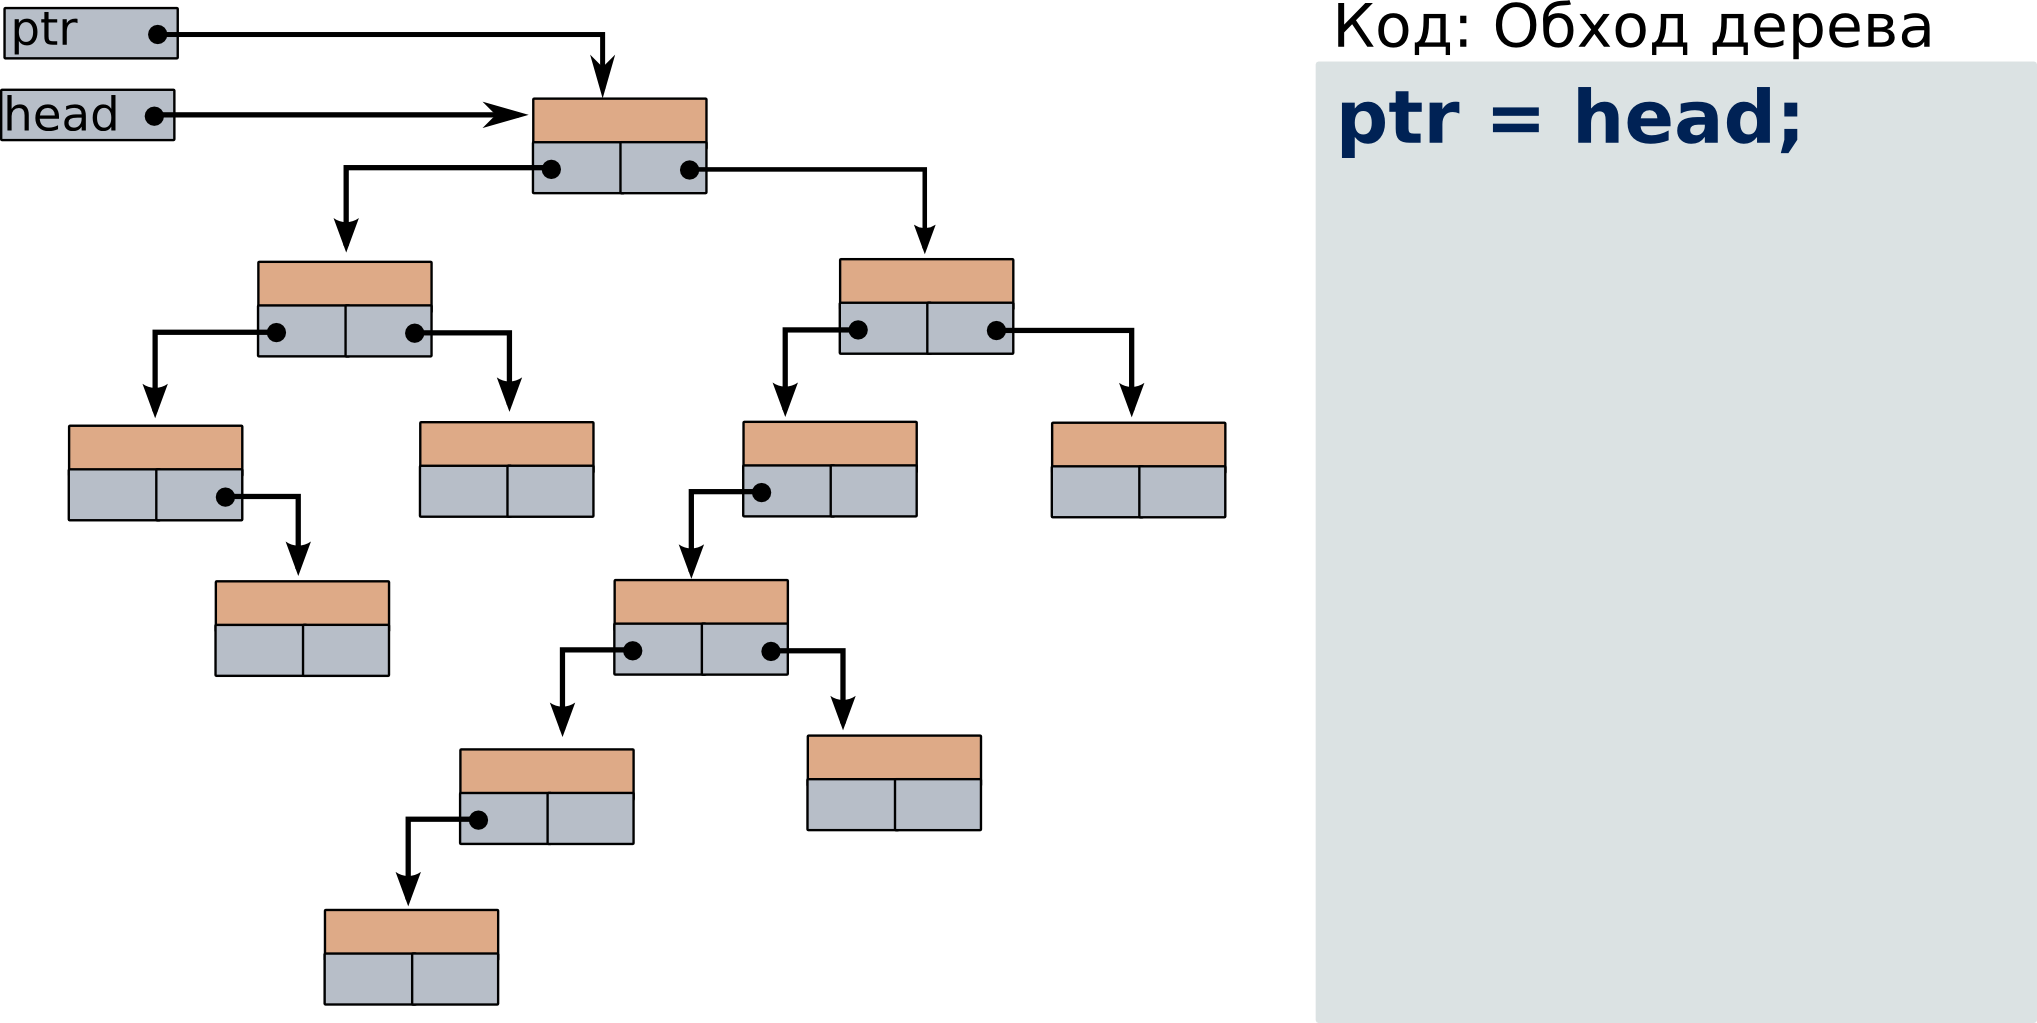
\includegraphics[width=0.99\linewidth]{images/bintree_traversal_1.png}
\end{center}
\end{frame}

\begin{frame}[fragile]
\frametitle{Двоичные деревья (обход)}  
\begin{center}
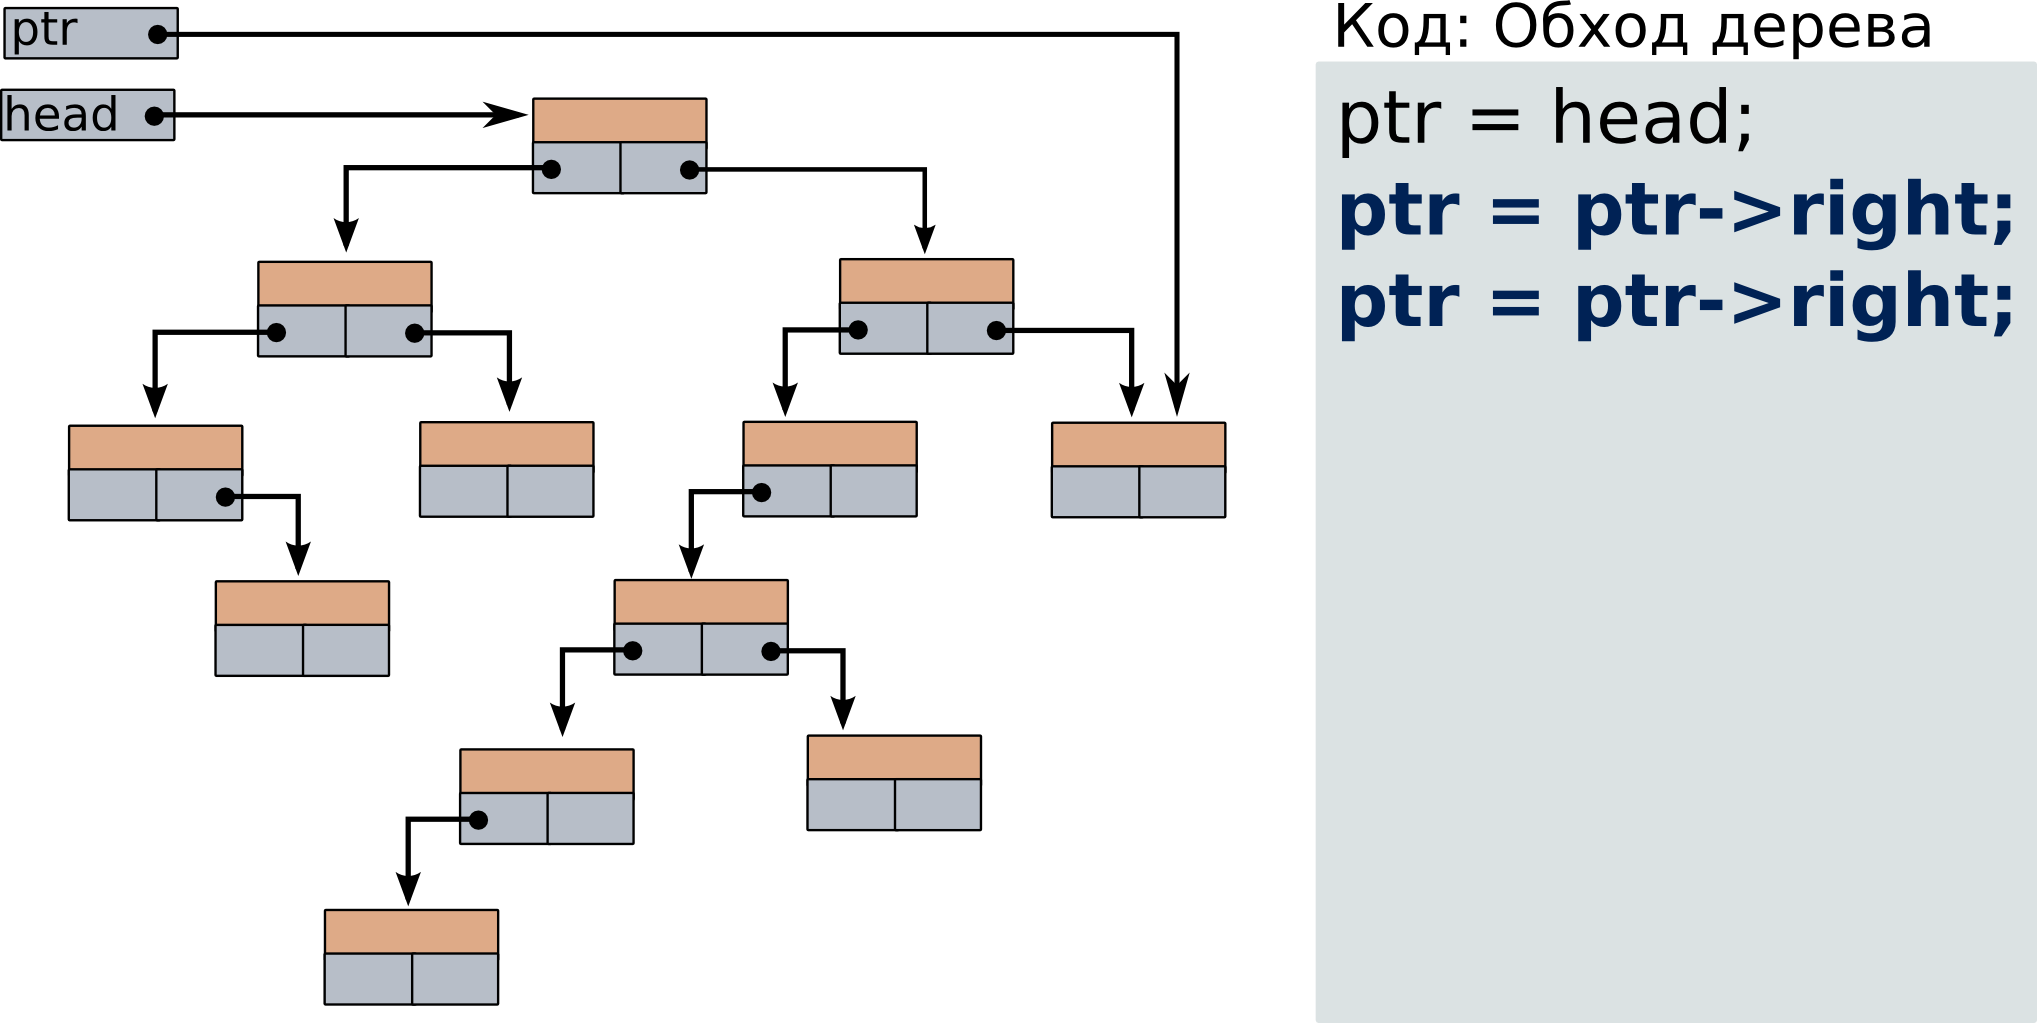
\includegraphics[width=0.99\linewidth]{images/bintree_traversal_2.png}
\end{center}
\end{frame}

\begin{frame}[fragile]
\frametitle{Двоичные деревья (обход)}  
\begin{center}
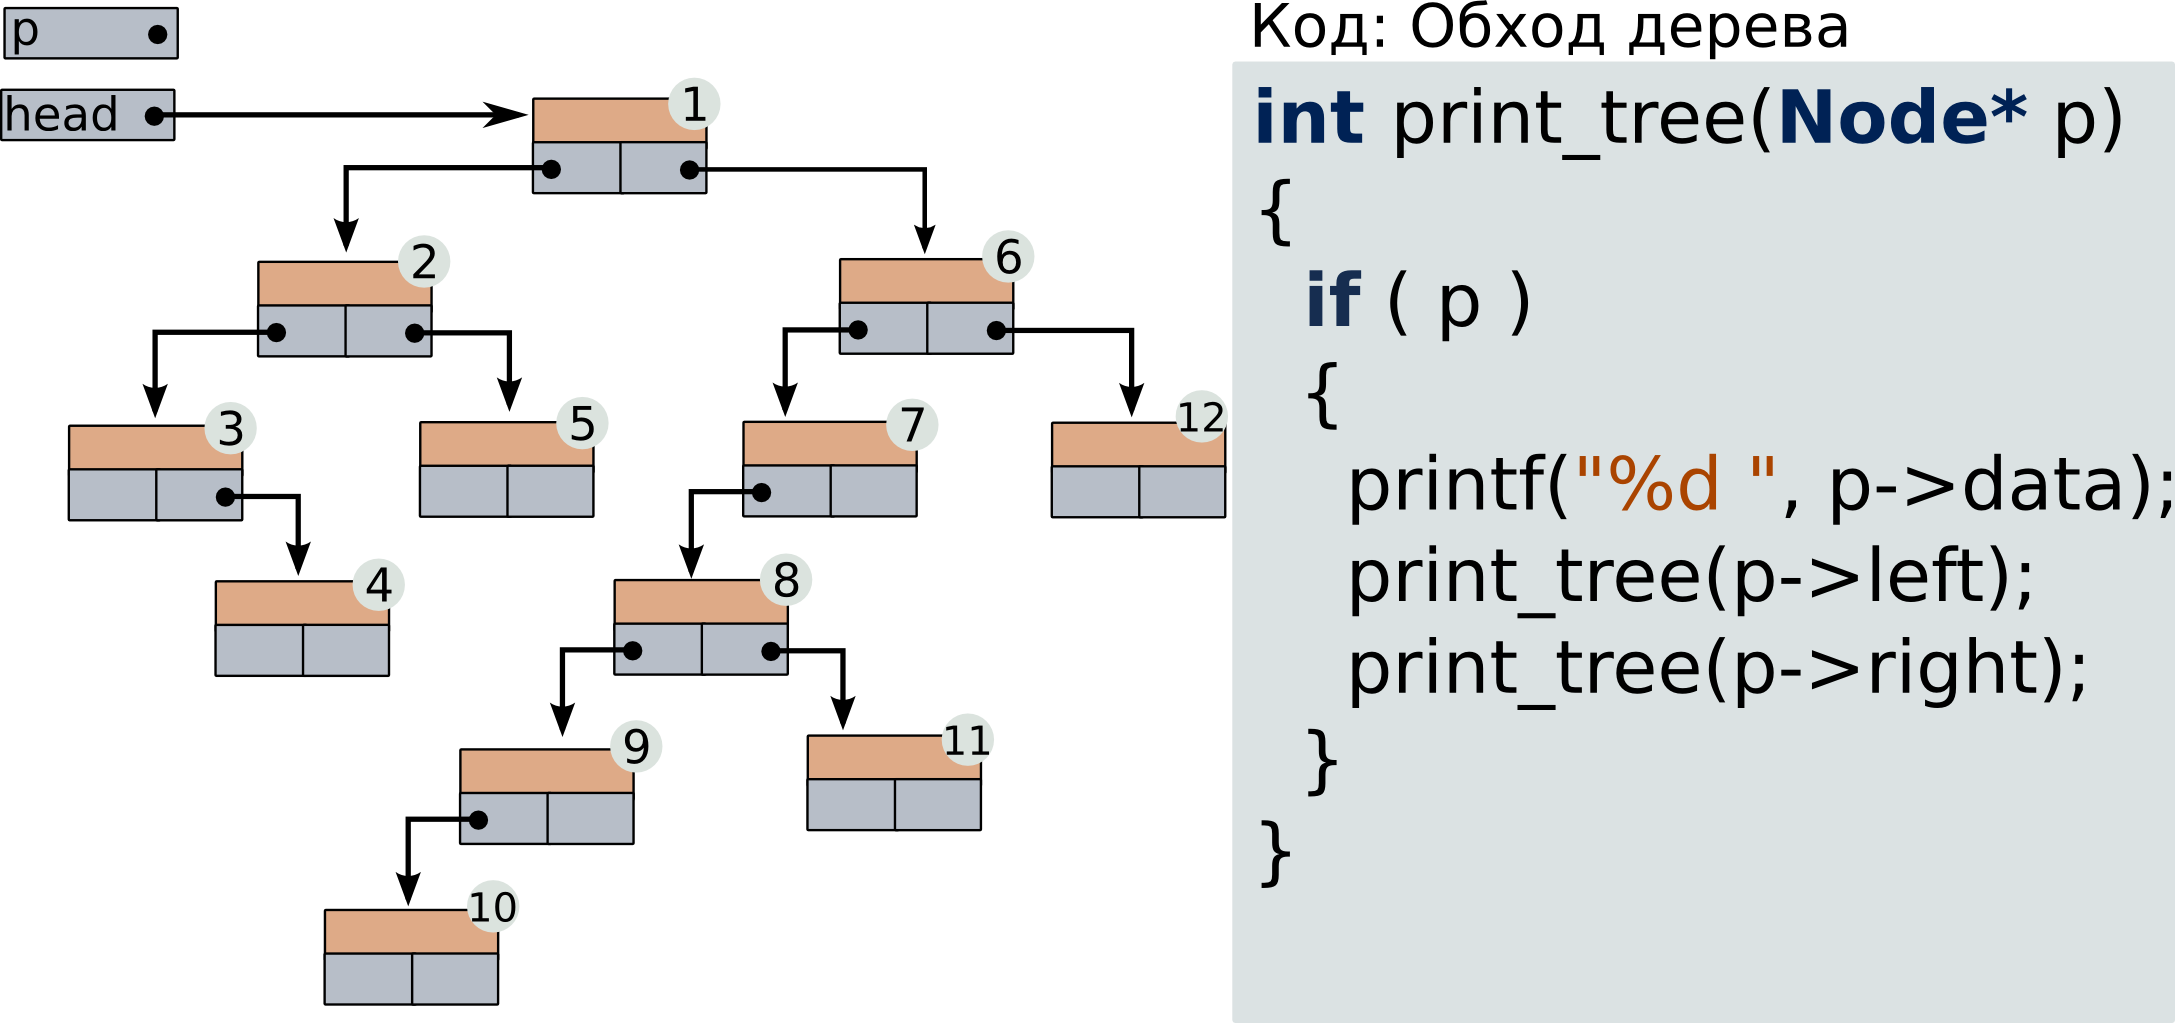
\includegraphics[width=0.99\linewidth]{images/bintree_traversal_3.png}
\end{center}
\end{frame}




\begin{frame}[fragile]
\frametitle{Двоичные деревья поиска} 
\begin{itemize}
\item Двоичные деревья поиска -- это двоичное дерево, обладающее следующим свойством:
\item Пусть $x$ -- произвольная вершина двоичного дерева поиска. Если вершина $y$ находится в левом поддереве
вершины $x$, то $y.data \leq x.data$. Если $y$ находится в правом поддереве вершины $x$, то $y.data \geq x.data$. 
\end{itemize}
\end{frame}

\begin{frame}[fragile]
\frametitle{Двоичные деревья поиска}  
\begin{center}
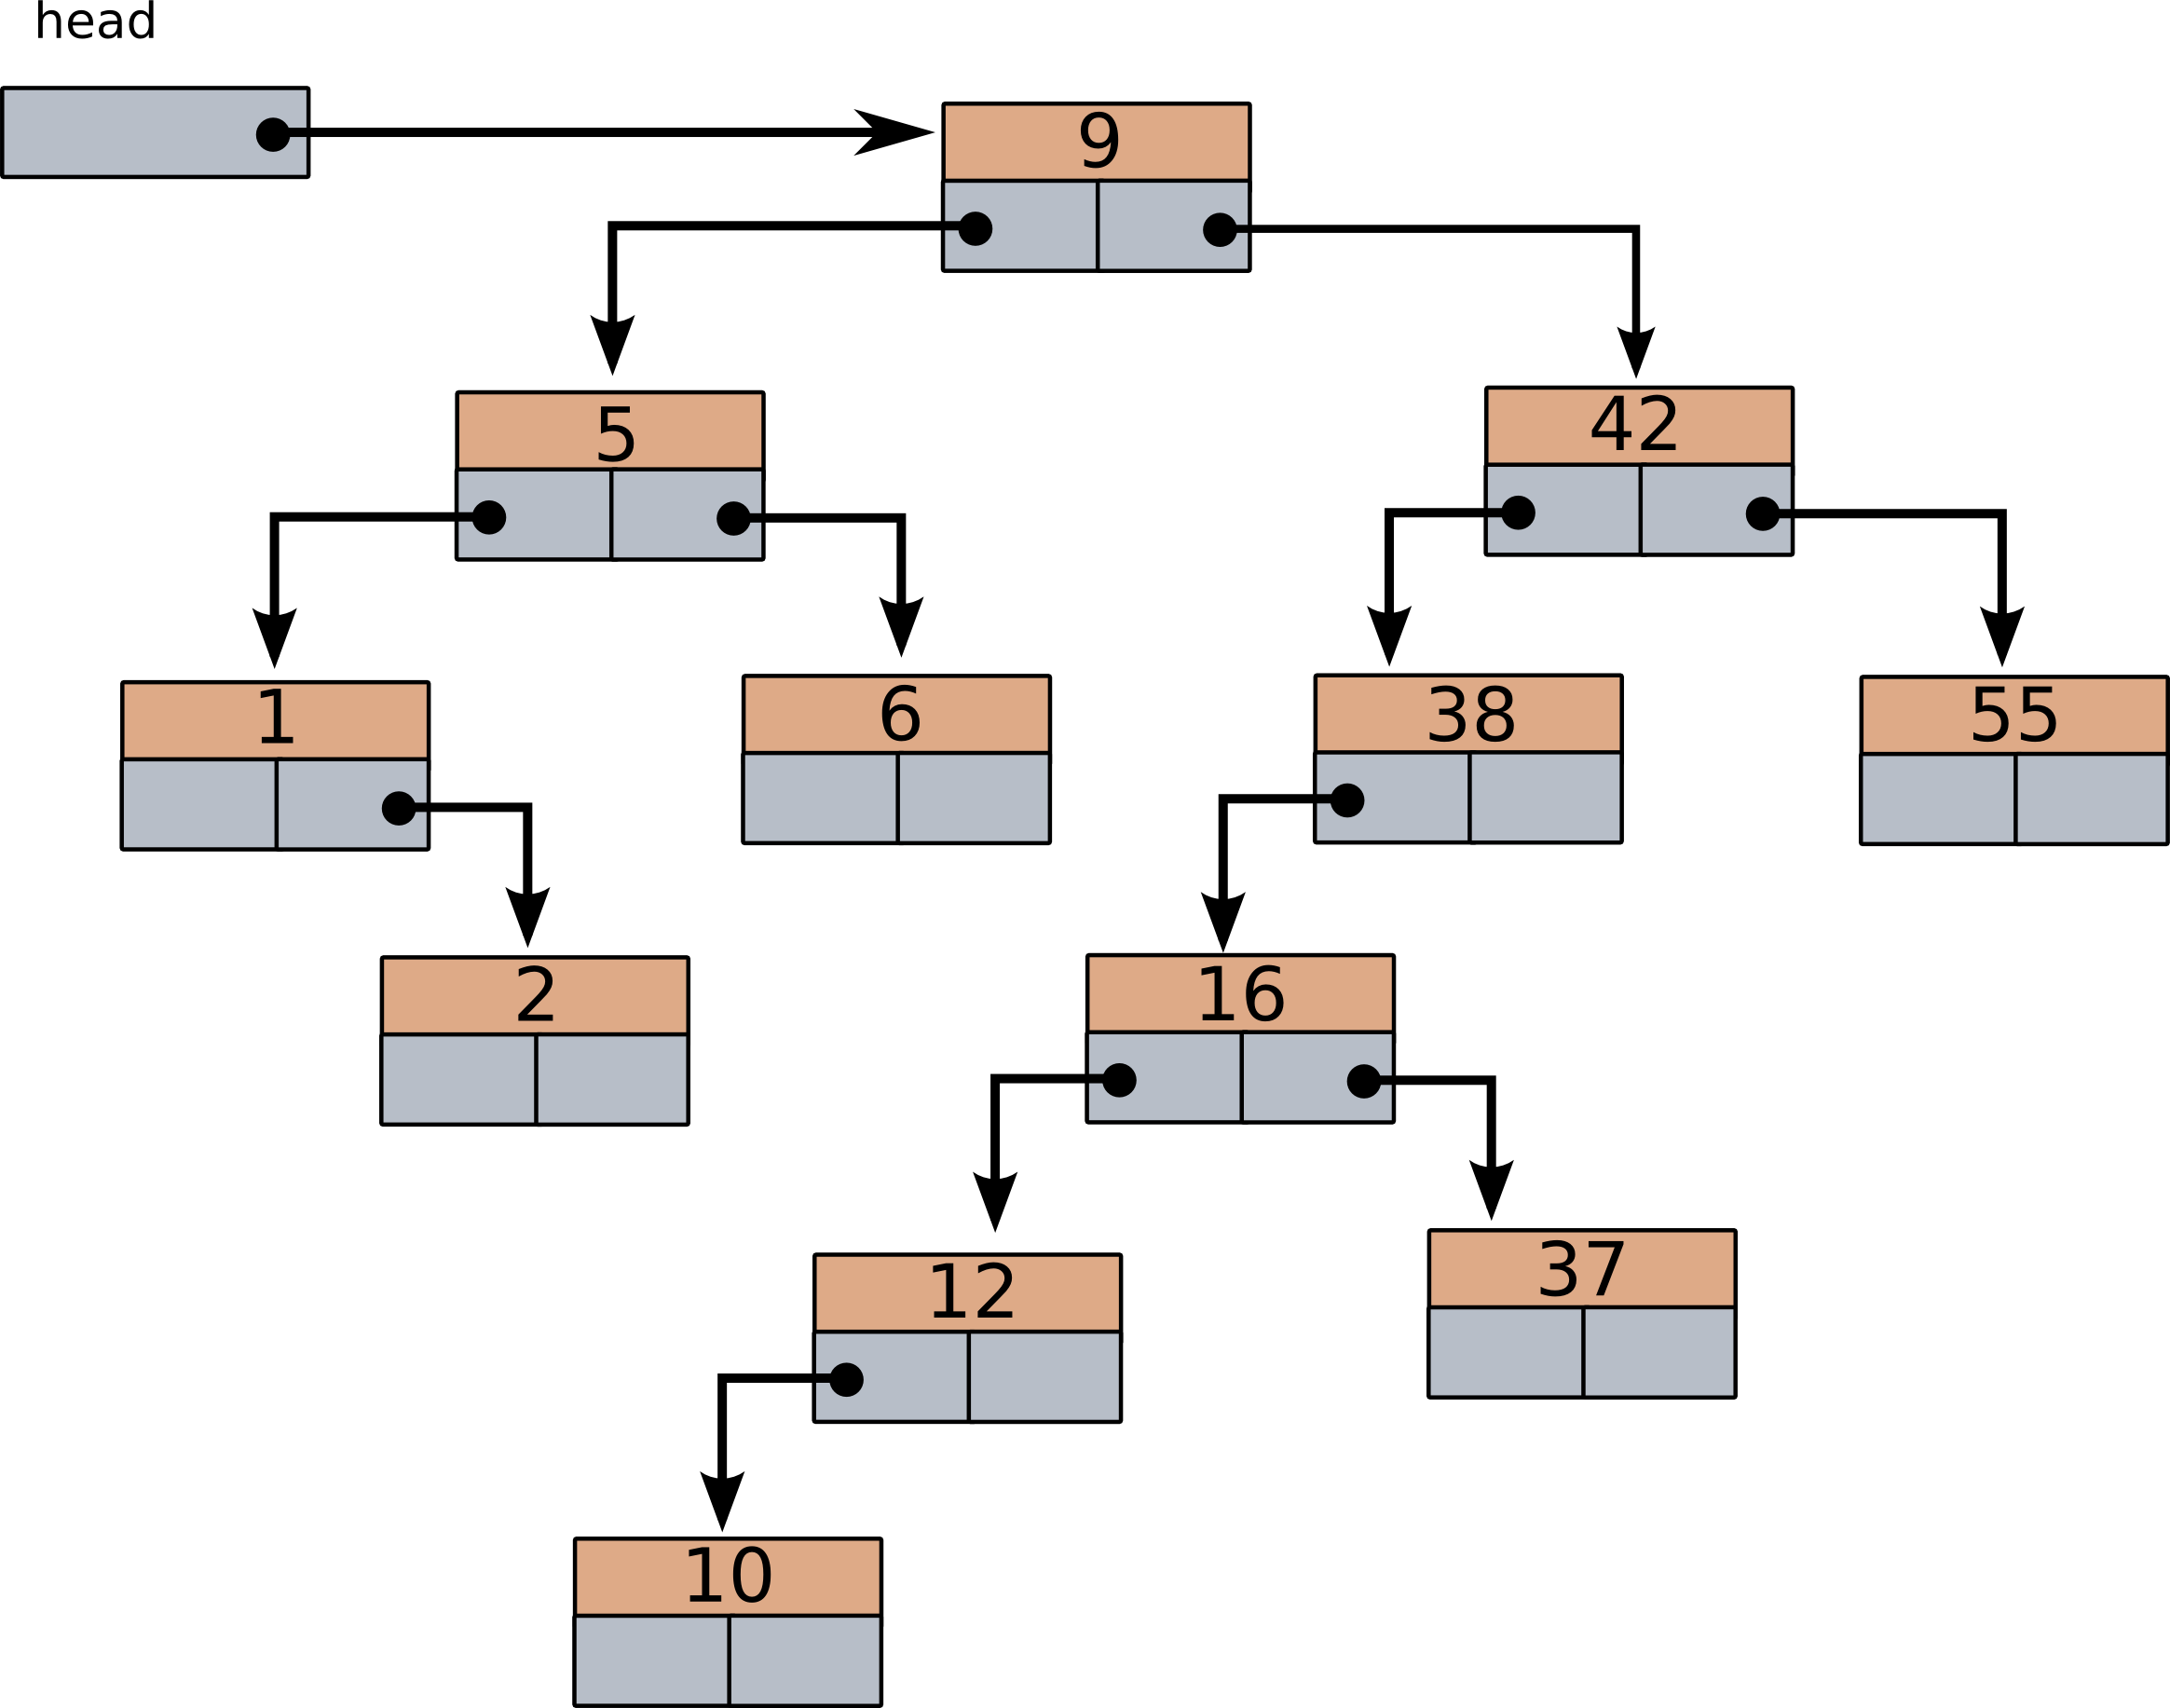
\includegraphics[width=0.75\linewidth]{images/bintree_search_1.png}
\end{center}
\end{frame}


\section{Запись/чтение файлов}
\begin{frame}
\begin{center}
\begin{beamercolorbox}[sep=8pt,center]{part
title}
\usebeamerfont{part title}\insertsection
\end{beamercolorbox}
\end{center}
\end{frame}

\begin{frame}[fragile]
\frametitle{Запись/чтение файлов} 
\begin{itemize}
\item Для работы с файлами нужно подключить заголовочный файл <stdio.h>
\item Создание указателя на файл:
\begin{lstlisting}
FILE * pFile;
\end{lstlisting}
\end{itemize}
\end{frame}

\begin{frame}[fragile]
\frametitle{Запись/чтение файлов} 
\frametitle{fopen и fclose} 
\begin{itemize}
\item Открыть файл:
\begin{lstlisting}
FILE *fopen(const char *filename, const char *mode);
\end{lstlisting}
\item Закрыть файл:
\begin{lstlisting}
int fclose(FILE *a_file);
\end{lstlisting}
\end{itemize}
\end{frame}

\begin{frame}[fragile]
\frametitle{Режмы работы с файлом} 
\begin{lstlisting}
FILE *fopen(const char *filename, const char *mode);
\end{lstlisting}
\begin{tabular}{ l || l }
  r & открыть существующий файл для чтения \\
  w & создать файл и открыть для записи \\
  a & открыть для записи в конец файла \\
  r+ & открыть для чтения/записи, с начала файла  \\
  w+ & создать файл и его открыть для чтения/записи \\
  a+ & открыть для чтения/записи в конец файла \\
\end{tabular}
\end{frame}

\begin{frame}[fragile]
\frametitle{fprintf, fscanf}  
\begin{lstlisting}[language=C++,basicstyle=\ttfamily,keywordstyle=\color{blue},
                stringstyle=\color{orange}\ttfamily]
   FILE *fptr;
   fptr=fopen("output.txt", "w");
   if(fptr==NULL){
      printf("Error!");   
      exit(1);             
   }
   fprintf(fptr, "%d", n);   
   fclose(fptr);
\end{lstlisting}
\end{frame}


\begin{frame}[fragile]
\frametitle{fputs, fgets}  
\begin{lstlisting}[language=C++,basicstyle=\ttfamily,keywordstyle=\color{blue},stringstyle=\color{orange}\ttfamily]
	FILE * f = fopen("input.txt", "r");
    
	int number_of_charss = 0;
	int c;

	while ((c = fgetc(f)) != EOF)
	{
	    number_of_charss++
	}
	fclose(f);
\end{lstlisting}
\end{frame}

\begin{frame}[fragile]
\frametitle{fread, fwrite}  
\begin{lstlisting}[language=C++,basicstyle=\ttfamily,keywordstyle=\color{blue},stringstyle=\color{orange}\ttfamily]
   char c[] = "some string data";
   char buffer[100];
   FILE *fp = fopen("output.txt", "w+");
   fwrite(c, strlen(c) + 1, 1, fp);
   fclose(fp);
\end{lstlisting}
\end{frame}





\section{Задание}
\begin{frame}
\begin{center}
\begin{beamercolorbox}[sep=8pt,center]{part
title}
\usebeamerfont{part title}\insertsection
\end{beamercolorbox}
\end{center}
\end{frame}

\begin{frame}[fragile]
\frametitle{Задание} 
\begin{itemize}
\item Тренировочная к/р №1, начать с wc-1
\end{itemize}
\end{frame}

\end{document}
